% Options for packages loaded elsewhere
\PassOptionsToPackage{unicode}{hyperref}
\PassOptionsToPackage{hyphens}{url}
%
\documentclass[
]{book}
\usepackage{amsmath,amssymb}
\usepackage{lmodern}
\usepackage{iftex}
\ifPDFTeX
  \usepackage[T1]{fontenc}
  \usepackage[utf8]{inputenc}
  \usepackage{textcomp} % provide euro and other symbols
\else % if luatex or xetex
  \usepackage{unicode-math}
  \defaultfontfeatures{Scale=MatchLowercase}
  \defaultfontfeatures[\rmfamily]{Ligatures=TeX,Scale=1}
\fi
% Use upquote if available, for straight quotes in verbatim environments
\IfFileExists{upquote.sty}{\usepackage{upquote}}{}
\IfFileExists{microtype.sty}{% use microtype if available
  \usepackage[]{microtype}
  \UseMicrotypeSet[protrusion]{basicmath} % disable protrusion for tt fonts
}{}
\makeatletter
\@ifundefined{KOMAClassName}{% if non-KOMA class
  \IfFileExists{parskip.sty}{%
    \usepackage{parskip}
  }{% else
    \setlength{\parindent}{0pt}
    \setlength{\parskip}{6pt plus 2pt minus 1pt}}
}{% if KOMA class
  \KOMAoptions{parskip=half}}
\makeatother
\usepackage{xcolor}
\usepackage{longtable,booktabs,array}
\usepackage{calc} % for calculating minipage widths
% Correct order of tables after \paragraph or \subparagraph
\usepackage{etoolbox}
\makeatletter
\patchcmd\longtable{\par}{\if@noskipsec\mbox{}\fi\par}{}{}
\makeatother
% Allow footnotes in longtable head/foot
\IfFileExists{footnotehyper.sty}{\usepackage{footnotehyper}}{\usepackage{footnote}}
\makesavenoteenv{longtable}
\usepackage{graphicx}
\makeatletter
\def\maxwidth{\ifdim\Gin@nat@width>\linewidth\linewidth\else\Gin@nat@width\fi}
\def\maxheight{\ifdim\Gin@nat@height>\textheight\textheight\else\Gin@nat@height\fi}
\makeatother
% Scale images if necessary, so that they will not overflow the page
% margins by default, and it is still possible to overwrite the defaults
% using explicit options in \includegraphics[width, height, ...]{}
\setkeys{Gin}{width=\maxwidth,height=\maxheight,keepaspectratio}
% Set default figure placement to htbp
\makeatletter
\def\fps@figure{htbp}
\makeatother
\setlength{\emergencystretch}{3em} % prevent overfull lines
\providecommand{\tightlist}{%
  \setlength{\itemsep}{0pt}\setlength{\parskip}{0pt}}
\setcounter{secnumdepth}{5}
\usepackage{booktabs}
\usepackage{amsthm}
\makeatletter
\def\thm@space@setup{%
  \thm@preskip=8pt plus 2pt minus 4pt
  \thm@postskip=\thm@preskip
}
\makeatother
\ifLuaTeX
  \usepackage{selnolig}  % disable illegal ligatures
\fi
\usepackage[]{natbib}
\bibliographystyle{apalike}
\IfFileExists{bookmark.sty}{\usepackage{bookmark}}{\usepackage{hyperref}}
\IfFileExists{xurl.sty}{\usepackage{xurl}}{} % add URL line breaks if available
\urlstyle{same} % disable monospaced font for URLs
\hypersetup{
  pdftitle={Introduction to Freight Transportation},
  pdfauthor={Scott S. Washburn, University of Florida, https://swash.essie.ufl.edu; Evangelos Kaiser, Florida Atlantic University, http://www.eng.fau.edu/directory/faculty/kaisar/; Lili Du, University of Florida, https://www.essie.ufl.edu/people/name/lili-du/},
  hidelinks,
  pdfcreator={LaTeX via pandoc}}

\title{Introduction to Freight Transportation}
\author{Scott S. Washburn, University of Florida, \url{https://swash.essie.ufl.edu} \and Evangelos Kaiser, Florida Atlantic University, \url{http://www.eng.fau.edu/directory/faculty/kaisar/} \and Lili Du, University of Florida, \url{https://www.essie.ufl.edu/people/name/lili-du/}}
\date{2023-04-18}

\begin{document}
\maketitle

{
\setcounter{tocdepth}{1}
\tableofcontents
}
\hypertarget{preface}{%
\chapter{Preface}\label{preface}}

This material is intended for an introduction to freight transportation course.Initial development of this material was sponsored by the Freight Mobility Research Institute (\url{http://eng.fau.edu/research/fmri/}).

An example figure is shown in Figure \ref{fig:PortImage}

\begin{figure}

{\centering \includegraphics[width=0.9\linewidth]{./Images/PortOfMiami} 

}

\caption{Port of Miami Partial Schematic}\label{fig:PortImage}
\end{figure}

\hypertarget{intro}{%
\chapter{Introduction}\label{intro}}

The movement of freight is a key foundation to the functioning of our society and economy\ldots{}

A sample math equation \(a^2 + b^2 = c^2\)

\hypertarget{intro-agencies}{%
\section{Applicable Federal Agencies}\label{intro-agencies}}

\begin{itemize}
\tightlist
\item
  BTS - Bureau of Transportation Statistics (\url{https://www.bts.gov/})
\item
  FHWA - Federal Highway Administration (\url{https://www.fhwa.dot.gov/})
\item
  FMCSA - Federal Motor Carrier Safety Administration (\url{https://www.fmcsa.dot.gov/})
\item
  NHTSA - National Highway Traffic Safety Administration (\url{https://www.nhtsa.gov/})
\item
  USDOT - United States Department of Transportation (\url{https://www.transportation.gov/})
\end{itemize}

\hypertarget{intro-statistics}{%
\section{Freight movement statistics}\label{intro-statistics}}

\textbf{Weight of shipments by transportation mode}

\begin{figure}

{\centering 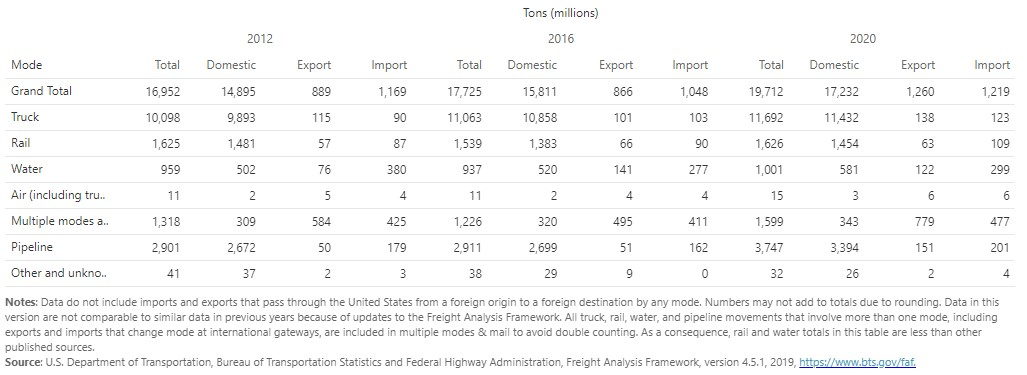
\includegraphics{./Images/FreightShipments_Weight} 

}

\caption{Weight of shipments by transportation mode}\label{fig:FreightByWeightImage}
\end{figure}

\textbf{Value of shipments by transportation mode}

\begin{figure}

{\centering 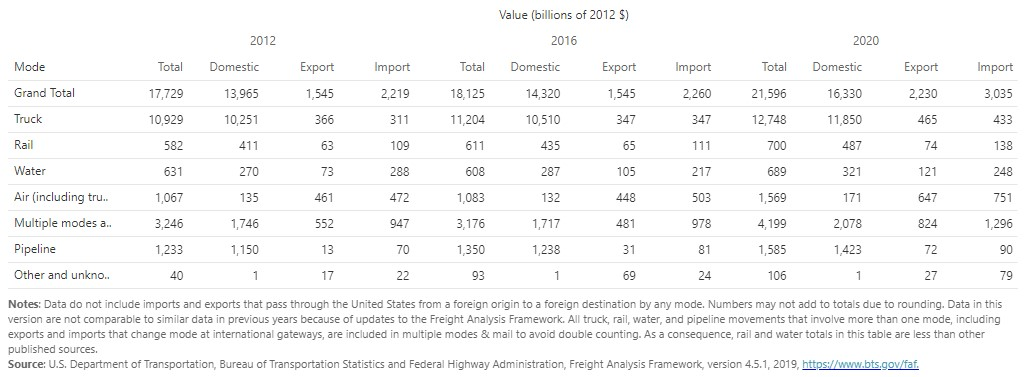
\includegraphics{./Images/FreightShipments_Value} 

}

\caption{Value of shipments by transportation mode}\label{fig:FreightByValueImage}
\end{figure}

Reference BTS

\hypertarget{VehChars}{%
\chapter{Freight Vehicle Characteristics}\label{VehChars}}

\hypertarget{VehChars-Classes}{%
\section{FHWA truck classifications}\label{VehChars-Classes}}

The FHWA designated vehicle classifications are shown in Figure \ref{fig:VehClassesImage}

\begin{figure}

{\centering 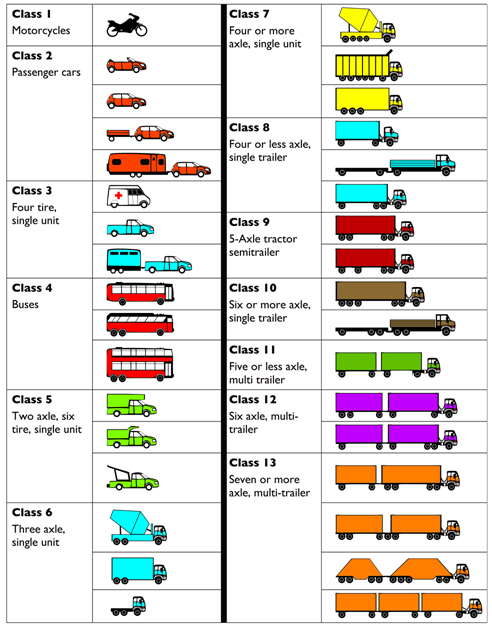
\includegraphics{./Images/VehClassesFHWA} 

}

\caption{FHWA Vehicle Classifications}\label{fig:VehClassesImage}
\end{figure}

Source: FHWA (2019). Traffic Monitoring Guide, Appendix C. Vehicle Types. USDOT. Washington, DC. URL: \url{https://www.fhwa.dot.gov/policyinformation/tmguide/tmg_2013/vehicle-types.cfm}.

\hypertarget{types-of-trailers}{%
\section{Types of trailers}\label{types-of-trailers}}

\begin{enumerate}
\def\labelenumi{\arabic{enumi}.}
\tightlist
\item
  Flatbed Trailer
\item
  Dry Vans
\item
  Refrigerated Trailer
\item
  Lowboy Trailers
\item
  Step Deck Trailers
\item
  Etc.
\end{enumerate}

\url{https://truckfreighter.com/tractor-types-trucks-trailers}

An example table is shown in Table \ref{tab:Example}

\begin{longtable}[]{@{}cc@{}}
\caption{\label{tab:Example} A sample table}\tabularnewline
\toprule()
Variable & Value (\%) \\
\midrule()
\endfirsthead
\toprule()
Variable & Value (\%) \\
\midrule()
\endhead
X & 25 \\
Y & 50 \\
Z & 75 \\
\bottomrule()
\end{longtable}

\hypertarget{performance-characteristics-accel-decel-speed-governing-etc.}{%
\section{Performance characteristics (accel, decel, speed governing, etc.)}\label{performance-characteristics-accel-decel-speed-governing-etc.}}

\hypertarget{unloaded-weights}{%
\section{Unloaded weights}\label{unloaded-weights}}

\hypertarget{geometric-design-considerations-turning-radius-sight-distance-etc.}{%
\section{Geometric design considerations (turning radius, sight distance, etc.)}\label{geometric-design-considerations-turning-radius-sight-distance-etc.}}

\hypertarget{loading-characteristics}{%
\chapter{Loading Characteristics}\label{loading-characteristics}}

\hypertarget{maximum-load-without-permit-max-load-with-permit-route-restrictions-time-of-day-restrictions}{%
\section{Maximum load without permit, max load with permit, route restrictions, time of day restrictions}\label{maximum-load-without-permit-max-load-with-permit-route-restrictions-time-of-day-restrictions}}

\hypertarget{weigh-stations-weigh-in-motion}{%
\section{Weigh stations, weigh-in-motion}\label{weigh-stations-weigh-in-motion}}

\hypertarget{driver-issues}{%
\chapter{Driver issues}\label{driver-issues}}

\hypertarget{hours-of-service}{%
\section{Hours of service}\label{hours-of-service}}

\hypertarget{training}{%
\section{Training}\label{training}}

\hypertarget{recruitment}{%
\section{Recruitment}\label{recruitment}}

\hypertarget{parking}{%
\chapter{Parking}\label{parking}}

\hypertarget{public-such-as-rest-areas}{%
\section{public, such as rest areas}\label{public-such-as-rest-areas}}

\hypertarget{private-such-as-travel-centers-of-americapetro}{%
\section{private, such as Travel Centers of America/Petro}\label{private-such-as-travel-centers-of-americapetro}}

\hypertarget{parking-availability-technologyinformation-systems}{%
\section{parking availability technology/information systems}\label{parking-availability-technologyinformation-systems}}

\hypertarget{port-issues}{%
\chapter{Port issues}\label{port-issues}}

\hypertarget{jayisha-das}{%
\section{Jayisha Das}\label{jayisha-das}}

Bureau of Transportation Statistics (2014). Freight Transportation. USDOT. Washington, DC. URL: \url{https://www.bts.gov/topics/freight-transportation}.

FHWA (2019). Traffic Monitoring Guide, Appendix C. Vehicle Types. USDOT. Washington, DC. URL: \url{https://www.fhwa.dot.gov/policyinformation/tmguide/tmg_2013/vehicle-types.cfm}.

Mannering, Fred L. and Washburn, Scott S. (2019). Principles of Highway Engineering and Traffic Analysis, 7th Edition. John Wiley and Sons, Hoboken, NJ.

Transportation Research Board (2016). Highway Capacity Manual, Sixth Edition: A Guide for Multimodal Mobility Analysis. Transportation Research Board, Washington, DC.

  \bibliography{references.bib}

\end{document}
